\documentclass[a4paper,12pt]{article}
\usepackage[top=1in, bottom=1in, left=1.2in, right=1.2in]{geometry}

\usepackage{url}
\usepackage{epsfig}
\usepackage{graphics}
\usepackage{fancyhdr}
\usepackage{graphicx}
\usepackage{parskip}
\usepackage[utf8]{inputenc}
\usepackage{float}
\usepackage{subcaption}
\usepackage[numbers]{natbib}
\usepackage{algorithm}
\usepackage[noend]{algpseudocode}
\usepackage{amsmath}

% Hifenização
\usepackage[brazil]{babel}
\usepackage[T1]{fontenc}
\hyphenation{pos-ta-gem si-lá-bi-ca}

\graphicspath{{pictures/}}

\title{Trabalho de Organização das Indústrias:\\ Plano de Negócios de uma empresa de Drones}
\author{\hspace*{-0.5cm}
\scalebox{0.7}{
    \begin{tabular}{cccccc}
        Artur Lemos & Daniel Guimarães & Fabrício Sander \\
        arturblemos@poli.ufrj.br & danielmguimaraes@poli.ufrj.br & fabriciosanderzubelli@poli.ufrj.br \\
        \\
        Ioav Lichtenstein & Jonas Degrave & Thiago Lobo \\
        ioav@poli.ufrj.br & jonasdegrave@poli.ufrj.br & thiagolobo@poli.ufrj.br \\
    \end{tabular}}
}
\date{}

\pagestyle{fancy}
\setlength{\headheight}{10pt}
\fancyhf{}
\lhead{Plano de Negócios - Organização das Indústrias}
\rhead{Grupo placeholder}
\cfoot{\thepage}

\begin{document}

\maketitle
\thispagestyle{fancy}

\section{Sumário Executivo}

Esse documento consiste no Plano de Negócios de uma empresa que atuará
no ramo de \emph{Drones} no mercado brasileiro. O mercado de multirotores
tem sofrido enormes crescimentos ao longo dos últimos 6 anos e ainda possui
muito potencial de desenvolvimento, tanto em termos tecnológicos quanto em
termos de aplicações. Não é incomum escutar comentários sobre empresas que
desejam realizar entregas de bens por meio de \emph{Drones} ou sobre filmes
que exibem cenas filmadas com eles, o que antes era feito com helicópteros,
de forma bastante mais cara.

O mercado de \emph{Drones} no Brasil ainda é bastante incipiente dado que
há muito pouca tecnologia sendo desenvolvida aqui, o que torna necessário
importá-la de países como China e Estados Unidos, principalmente.
Isso acarreta aumentos de custos por impostos alfandegários e limita
aplicações, já que o consumidor está preso à visão dos produtores dos países
supracitados e às suas plataformas "fechadas".

O objetivo da empresa é, então, produzir e comercializar o componente mais caro 
e importante de qualquer aeronave: o controlador de voo. Além disso, desejamos
também oferecer serviços nas áreas de sensoriamento remoto, fotografia, mapeamento
de terreno 2D (georreferenciamento) e 3D e em quaisquer outras novas áreas onde
a tecnologia seja aplicável de forma eficiente, também sob demanda de clientes.

O documento está estruturado de forma que apresentará os seguintes componentes:

\begin{itemize}
	\item Análise de Mercado
	\item Plano de Gestão
	\item Plano de Marketing
	\item Plano Operacional
	\item Plano Financeiro
	\item Conclusão
\end{itemize}

% SEBRAE diz pra colocar essas coisas no sumário executivo, mas acho melhor
% distribuir ao longo do documento, onde faça sentido colocar cada coisa:

% \begin{itemize}
% 	\item O que é o negócio
% 	\item Principais produtos e serviços
% 	\item Principais clientes
% 	\item Localização
% 	\item Capital a ser investido
% 	\item Faturamento mensal
% 	\item Lucro
% 	\item ROIs
% 	\item CPF/CNPJ
% 	\item Sócios
% 	\item Missão da empresa
% 	\item Setores de atividades
% 	\item Forma jurídica: Sociedade Limitada
% 	\item Capital social
% 	\item Fontes de recursos
% \end{itemize}



\section{Análise de Mercado}

\subsection{Estudo dos Clientes}

A empresa atenderia, potencialmente, pessoas físicas e jurídicas, dividindo a possível clientela em termos
dos dois principais produtos: o controlador de voo e a prestação de serviços.

\subsubsection*{Controlador de Voo}

Provavelmente apenas pessoas físicas de um nicho bastante específico: \emph{hobbystas}. Vender um controlador de voo com sua máxima capacidade de atuação e customização seria ingênuo, já que permitiria que terceiros utilizassem-no para prestar serviços, o que reduziria nossa fatia de clientes. Considerando-se isso, desejamos vender uma versão do controlador que permita fazer o mínimo necessário para voos recreativos e filmagens simples, de forma a competir com os produtos de empresas estrangeiras no que diz respeito a preços. Esse mercado já possui elevado potencial, segundo nossas pesquisas.

O controlador de voo seria direcionado a \emph{hobbystas} pois exige conhecimento razoavelmente avançado para ser utilizado. Não é um produto que funcionará \emph{out of the box}, dado que é necessário montar todo o resto do multirotor, acoplar o controlador a ele e calibrá-lo. Esse público é composto, majoritariamente, por homens de faixa etária acima de 15 anos, com média de aproximadamente 30 anos. Vale ressaltar que o limite inferior de faixa etária tende a diminuir, dado o crescente e fácil acesso a informações bastante técnicas e específicas disponibilizado pela internet.

Quanto ao ramo de atuação da clientela, a probabilidade é que encontremos mais pessoas inclinadas ao lado das disciplinas exatas, devido ao fator técnico do produto. Porém, o público não é restrito a profissinais dessa área. Encontramos, em nossas pesquisas, pessoas da área do Direito e da Medicina, por exemplo. Fato é que o poder aquisitivo do público alvo tem de ser razoavelmente alto, dados os preços de montagem e manutenção dessas plataformas. Um ponto interessante é que \emph{hobbystas} tendem a levar a prática bastante a sério, tornando-se clientes assíduos e leais, dispostos a pagar quantias altas ao encontrarem produtos que julguem interessantes. Falamos isso também por experiência própria. O nível de escolaridade da clientela tende, também, a ser alto: provavelmente, no mínimo, Ensino Médio Técnico completo. Clientes desse tipo são encontrados em todo o país, principalmente nas grandes cidades, como Rio de Janeiro ou São Paulo.

A probabilidade de um \emph{hobbysta} comprar o produto mais do que uma vez não é tão alta, porém não é nula. Por outro lado, reiterações do produto (versões novas) tendem a atrair o público, que é leal, como citado anteriormente. Atualmente, esse público se dispõe a pagar de R\$ 800.00 a 1200.00 nesse componente (modelo Naza V2 da concorrente DJI). As vendas podem ser feitas \emph{online}, com envio pelos \emph{Correios}, já que o produto é bastante pequeno.

\subsubsection*{Prestação de Serviços}

A prestação de serviços é o produto que atingirá o maior público alvo, também gerando a maior parcela de faturamento da empresa. Como dito anteriormente, aplicações para \emph{Drones} surgem a cada dia, potencialmente otimizando e reduzindo custos de certas atividades.

Aqui, o maior faturamento virá provavelmente de prestação de serviços à empresas. A ideia é adaptar o controlador de voo base para uma versão customizada a cada cliente. O controlador básico permite que a aeronave voe de forma estável e autônoma, com rotas pré-programadas ou controle manual. Com isso, podemos, por exemplo, permitir transmissão de imagem em tempo real e \emph{logging} de coordenadas de GPS para mapear a área de um terreno agrícola. Outra aplicação seria coletar dados de forma remota: pode-se acoplar quaisquer sensores à aeronave, permitindo, por exemplo, que uma empresa que deseja instalar painéis solares navegue com o \emph{Drone} ao longo do terreno, medindo a incidência média de luz do sol (e outras variáveis como temperatura, umidade etc) e, em seguida (ou em tempo real), obtenha um mapa com os dados explicitados, possibilitando escolher pontos que maximizem a incidência para realizar a instalação.

Empresas que trabalhem com engenharia civil, inspeções em geral, fotografia, filmagem dentre outras áreas também se beneficiariam da tecnologia. Pessoas físicas provavelmente se utilizariam de aplicações semelhantes às empresas porém em menor escala, de forma que as quantias de dinheiro envolvidas serão menores. Os serviços terão frequência de "reincidência"\ variável: é mais provável que pessoas físicas demandem mais filmagens de casamentos do que empresas demandem coletas de incidência solar, por exemplo. Por outro lado, o projeto de uma empresa tem nível de complexidade maior, exigindo \emph{software} adicional para interação com a aeronave, assistência e talvez a venda da aeronave, especializada para certa aplicação, como um todo, junto à assistência de como utilizá-la. Preços de serviços de fotografia ou filmagem podem variar de R\$ 200.00 a 2000.00, para grandes eventos, com possíveis transmissões ao vivo, diversos ângulos, câmeras melhores etc. Serviços diversos, na área de mapeamento ou sensoriamento, com ou sem a venda da plataforma, podem variar de R\$ 1000.00 a 30000.00 ou mais, dependendo do projeto.

A depender da magnitude do projeto, pode haver deslocamento da equipe para prestação de serviço, porém almejamos iniciar com serviços no interior de São Paulo, onde há grande concentração de instalações agrícolas comerciais.

\subsection{Estudo dos Concorrentes}

O principal concorrente é certamente a chinesa DJI, com seu famoso \emph{Drone} Phantom, atualmente na quarta iteração. De qualidade excepcional, oferece grande facilidade de uso, tempo de voo acima da média, estabilidade excelente e filmagens e fotos de ótima qualidade. A empresa também oferece seu controlador de voo, o Naza V2 para entusiastas e \emph{hobbystas} que desejam a mesma estabilidade numa plataforma diferente. Como o produto é de origem chinesa, é possível encontrá-lo em terras brasileiras, por meio de revendedores, por cerca de R\$5500.00 (Phantom) e R\$ 1000.00 (Naza V2). Mesmo com os altos preços, é notório o público que se dispõe a comprar o produto.

A nossa vantagem em comparação com a DJI é apostar na área de prestação de serviços. A plataforma da empresa chinesa é totalmente fechada, direcionada única e exclusivamente a um usuário final médio, com pouco conhecimento na área, disposto a adquirir um "brinquedo"\ avançado. Existem empresas que empregam o Phantom em prestação de serviços, porém de forma limitada à captura de imagens, que é o máximo oferecido pela DJI. Há uma crescente comunidade que visa modificar o Phantom para permitir novas capacidades, porém imaginamos que um produto criado com uma aplicação em mente dificilmente se adapta tão bem a outra aplicação.

Na área de prestação de serviços, há uma crescente onda de empresas brasileiras que utilizam \emph{Drones} comerciais (como o Phantom) para aplicações que envolvem captura de imagens. Porém, nenhuma dessas empresas detém tecnologia própria. Como mencionado anteriormente, o Brasil ainda é extremamente pobre no que diz respeito à geração de tecnologia nessa área. Isso limita as empresas brasileiras às aplicações pensadas originalmente pelas empresas do exterior, de forma que enxergamos aí um espaço para, junto ao cliente, encontrar uma solução maximamente otimizada na forma de um controlador de voo especializado. 

\subsection{Estudo dos Fornecedores}

Não só não existe produção de controladores de voo no Brasil, como tamém não existe produção dos outros componentes de um \emph{Drone}. Isso inclui a estrutura (essa é a mais facilmente substitutível por um produto brasileiro, já que não exige tecnologias muito avançadas), os motores elétricos, as baterias, os controladores de velocidade dos motores etc.

Isso implica que teremos que importar peças, por exemplo, através do \emph{AliExpress}. Como nosso intuito não é primariamente o de vender \emph{Drones} (e caso isso seja necessário, incluiremos o custo da plataforma no custo do serviço), teremos que manter algumas plataformas próprias, cujo número aumentará com o crescimento da empresa, porém não muito rapidamente. Um estoque de segurança deverá ser mantido, levando em conta o fato de que entregas pelo \emph{AliExpress} costumam levar meses.

Quanto ao controlador de voo, teremos que encontrar fornecedores de placas de circuito impresso para realizarem a impressão do nosso design e, talvez, a soldagem dos componentes. Para tanto, entraremos em contato com as empresas que desenvolvem os componentes do controlador (microcontrolador e sensores), como: Bosch, ATMEL, InvenSense, U-Blox etc e negociaremos compras em quantidades elevadas dos componentes, considerando tempo de entrega e custos.
\section{Plano de Gestão}

O objetivo dessa seção é estruturar com maior clareza a estratégia de atuação da empresa,
levando em conta micro e macroaspectos que influenciam em seu desempenho. Para tanto, serão 
feitas duas análises: CAMGPEST e fatores críticos de sucesso. A primeira análise consiste num 
diagnóstico dos macrofatores culturais, ambientais, mercadológicos, geográficos, políticos, 
econômicos, sociais e tecnológicos que dizem respeito ao escopo da empresa. Já o segundo método 
realiza um diagnóstico dos pontos fortes e fracos dos fatores mais relevantes aos principais 
concorrentes.

\subsection{Análise CAMGPEST}

\subsubsection*{Fatores Culturais}

Drones têm entrado cada vez mais na cultura popular ao redor do mundo. Até mesmo no Brasil, 
onde a tecnologia costuma chegar com certo atraso, observam-se estatísticas de compras crescentes, 
principalmente no ramo de drones "populares", ou seja, prontos para voar out-of-the-box, porém com 
aplicações limitadas à obtenção de imagens aéreas amadoras e entretenimento \cite{brasildrones}. 
O exemplo mais notório desse tipo de drones é, 
certamente, o Phantom, atualmente em sua quarta iteração, da concorrente chinesa DJI.

A difusão global desse tipo de aeronaves, respaldada por taxas de aumentos de vendas mundiais 
como a entre os anos de 2014 e 2015, quando o aumento foi de 63\% \cite{dronestats}, certamente 
mostra-se benéfica para a empresa. Com um público que conhece drones cada vez maior, cria-se, 
primariamente, um ambiente propício à prestação de serviço com essa tecnologia e, secundariamente, 
um público hobbysta crescente.

\subsubsection*{Fatores Ambientais}

Como será descrito no Plano de Marketing, a tecnologia de Drones permite diversos impactos positivos 
no que diz respeito ao meio-ambiente. Como uma das áreas de prestação de serviços de maior potencial 
é a obtenção de imagens agrícolas aéreas, pode-se, consequentemente, monitorar processos de recuperação 
ambiental, avaliar danos ambientais e desmatamento, encontrar e delimitar incêndios de modo eficiente e 
monitorar pragas. Ademais, a fonte de energia das aeronaves é bastante mais vantajosa do que combustíveis 
fósseis, no que tange a emissão de poluentes, que é essencialmente nula, nesse caso.

\subsubsection*{Fatores Mercadológicos}

Clientes potenciais, sob o ponto de vista da empresa, são, primariamente, atuantes dos seguintes setores:

\begin{itemize}
	\item Agrícola: proprietários de fazendas e de grandes áreas que exigem qualquer tipo de inspeção
	\item Ambiental: institutos de licenciamento e gerenciamento de recursos ambientais e naturais, como o IBAMA
	\item Engenharia Civil: construtoras ou órgãos de defesa civíl, os quais se beneficiariam da obtenção de 
	imagens para inspeção
	\item Indústria Cinematográfica: todo o público interessado em formas de se obter imagens aéreas com custos reduzidos e 
	maior flexibilidade para fins de entretenimento
	\item Hobbystas: foco do controlador de voo, cuja vantagem há de ser a oferta de capacidades semelhantes às dos 
	concorrentes sob menor custo
\end{itemize}

\subsubsection*{Fatores Geográficos}

Uma das maiores vantagens da empresa advém da dificuldade (que se apresenta em forma de altos preços) 
de atuação de empresas do exterior, as quais usualmente detém esse tipo de tecnologia, no Brasil. Essa 
vantagem se expressa, principalmente, no setor de prestação de serviços com Drones, o qual é extremamente 
carente de atuantes internacionais. Quanto ao controlador de voo, pode-se praticar preços menores, isentos 
dos enormes impostos alfandegários praticados no país.

\subsubsection*{Fatores Políticos}

Devido à natureza da empresa, sua atuação não expressará impactos políticos importantes além de, 
possivelmente, fomentar desenvolvimento tecnológico em território nacional, também com a venda dos controladores de voo.

\subsubsection*{Fatores Econômicos}

A atuação da empresa se vê beneficiada pela situação econômica do país de duas formas, levando em 
conta a atual situação de recessão. 

Primeiramente, quanto à prestação de serviços, os clientes potencialmente aumentarão seus lucros 
ao utilizarem-se da tecnologia oferecida. Um exemplo disso é na agricultura: com a obtenção de 
imagens aéreas por meio de drones (cujo custo de operacional é bastante menor que o de helicópteros 
e satélites), um produtor pode saber, de forma bastante precisa, o número de unidades plantadas e, 
consequentemente, a quantia de pesticida a ser utilizada sem grandes desperdícios. Além disso, uma 
construtora pode inspecionar certa área de difícil acesso de uma obra sem ter de colocar um operário 
em atividade de risco, o que acarreta altos custos.

Secundariamente, no ramo das vendas do controlador de voos, temos, outra vez, o baixo custo como 
principal vantagem. Além disso, com o crescimento da classe média observado ao longo dos últimos 
dez anos, pode-se esperar um público hobbysta expressivo com interesses no produto.

\subsubsection*{Fatores Sociais}

Devido à natureza da empresa, não esperam-se impactos sociais expressivos.

\subsubsection*{Fatores Tecnológicos}
	
Os objetivos da empresa são altamente correlacionados à tecnologia. Podem-se enumerar diversas influências 
positivas da área na produção do controlador de voo e na prestação de serviços. 

Quanto ao controlador de voo, é notória a importância do desenvolvimento tecnológico. A crescente 
miniaturização de componentes com desempenho de processamento cada vez melhor, aliada à disponibilidade 
de sensores cada vez mais precisos e confiáveis permite o desenvolvimento de controladores cujo desempenho 
viabiliza estabilidade excepcional, mantendo a massa da aeronave mínima, permitindo que o usuário adicione 
outros dispositivos, conforme a aplicação almejada. Uma área que tem crescido muito ao longo da última década, 
a Inteligência Artificial, potencialmente contribuirá muito no controle de voo de aeronaves, permitindo 
tomada de decisões autônoma e uso mais eficiente de recursos energéticos.

A prestação de serviços será mais eficiente à medida que o controlador de voo for mais eficiente. Porém, 
essa área também será beneficiada por tecnologias periféricas. Um exemplo disso é o desenvolvimento de 
aplicativos para tablets, permitindo interação e visualizações rápidas dos dados coletados pelo drone com 
mapas de relevo 3D, georreferenciamento com coordenadas de GPS etc.

\subsection{Análise de Fatores Críticos de Sucesso}

Essa análise utiliza um sistema de pontuação para comparar a empresa aos seus principais concorrentes de 
forma a identificar suas vantagens competitivas e desvantagens que precisam ser trabalhadas.

Como a empresa se propõe a atender dois mercados bastantes distintos, duas comparações serão realizadas, 
uma em relação ao mercado hobbysta e outra em relação à prestação de serviços.

A seguir, a primeira tabela é apresentada com os principais fatores críticos de sucesso em relação ao 
mercado de serviços:

%tabela aqui

Pode-se observar que a respeito do mercado de prestação de serviço a capacidade da empresa desenvolver 
o hardware dos drones utilizados \emph{in-house} a permite oferecer preços mais baixos do que os concorrentes 
que utilizam drones comerciais. Além disso, o acesso ao hardware permite que a empresa ofereça serviços mais 
personalizados a diferentes clientes, tendo a capacidade de alterar o comportamento do drone sob medida. 
Por outro lado, por ser uma nova ingressante no mercado, a marca da empresa não possuirá reconhecimento. 
Ademais, uma empresa pequena não será capaz de oferecer serviços a muitos clientes simultâneos nem equipamentos 
de tão alto desempenho quanto os desenvolvidos pelas empresas líderes do mercado.

A tabela abaixo descreve os fatores críticos de sucesso em relação ao mercado hobbysta:

%tabela aqui

A respeito do mercado hobbysta, a produção nacional permite à empresa produzir um equipamento com preço 
mais baixo, com qualidade similar ou pouco inferior ao importado. No caso de um hobbysta mais dedicado, 
há ainda a possibilidade, proporcionada pela proximidade no mercado nacional, do desenvolvimento de soluções 
personalizadas.

Novamente, o reconhecimento no mercado é uma fragilidade inicial que precisa ser considerada. Além disso, 
os fabricantes tradicionais oferecem uma gama maior de produtos, tem maior capacidade produtiva e são 
capazes de desenvolver equipamentos de mais alto desempenho.
\section{Plano de Marketing}

\subsection{Descrição dos produtos e serviços}

\subsubsection*{Controlador de Voo}

O controlador de voo consiste num dispositivo de aproximadamente 
$7$ x $3$ x $1.5$ $cm^3$, o qual inclui diversas entradas e saídas, 
como no diagrama a seguir:

\begin{figure}[H]
\centering
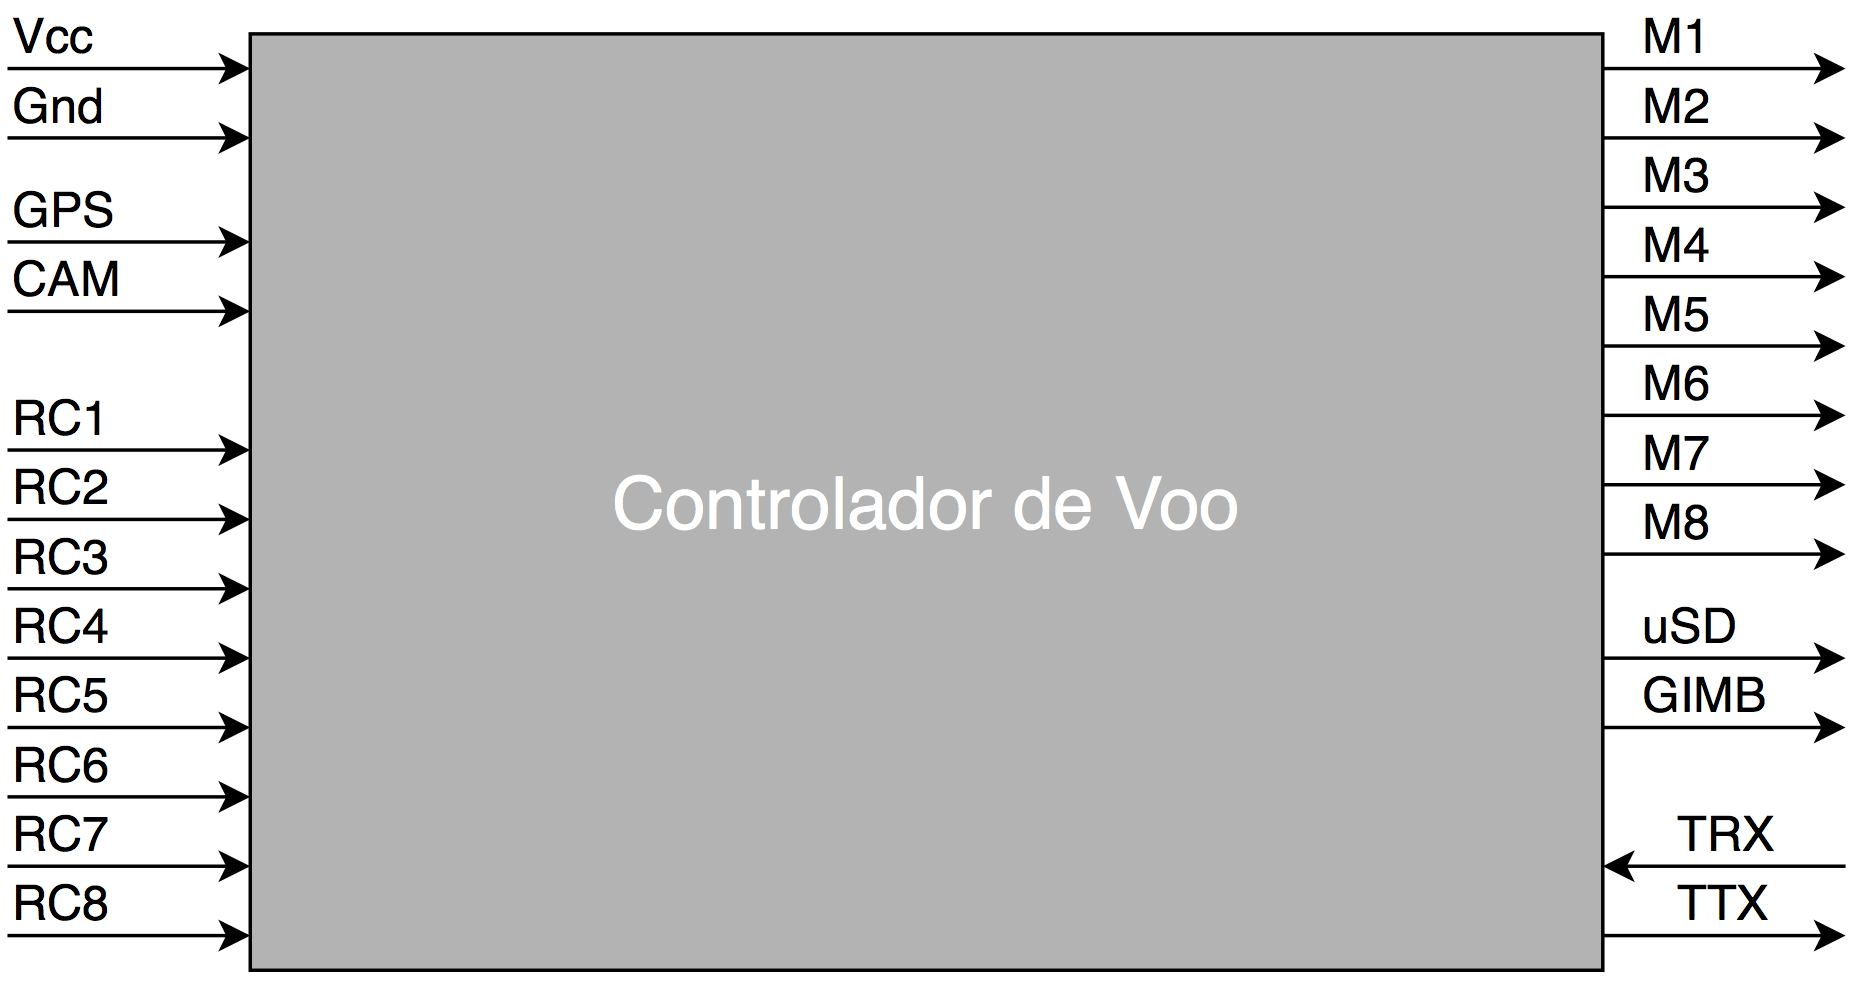
\includegraphics[width=\textwidth]{fcdiagrama.png}
\caption{Diagrama de entradas e saídas do controlador de voo.}
\label{fig:fcdiagrama}
\end{figure}

Descrição das entradas e saídas:
\begin{itemize}
	\item Vcc: Alimentação +12 Volts
	\item Gnd: Alimentação terra
	\item GPS: Entrada de dados de módulo de GPS
	\item CAM: Entrada de dados de módulo de câmera
	\item RC1..RC8: Entrada de dados de cada um dos 8 possíveis 
	canais de rádio controle
	\item M1..M8: Saídas de comandos para cada um dos possíveis 8 motores
	\item uSD: Saída de dados para cartão SD (caixa preta)
	\item GIMB: Saída de comandos para \emph{Gimbal} (sistema de estabilização de câmera)
	\item TRX: Entrada de dados de \emph{link} digital de telemetria
	\item TTX: Saída de dados de \emph{link} digital de telemetria
\end{itemize}

Internamente, o controlador possui um microcontrolador que é 
responsável pela execução do \emph{firmware} de controle, giroscópio 
3D (ou seja, nos eixos $x, y$ e $z$), acelerômetro 3D, magnetômetro 
3D, barômetro e termômetro. O mínimo necessário para voar é um rádio
controle de 4 canais, uma bateria de polímero de lítio para 
alimentação do \emph{drone} inteiro e ao menos 4 motores.

Caso o usuário deseje, pode-se conectar um módulo de GPS externo, 
permitindo navegação autônoma baseada em coordenadas; um cartão
SD para permitir gravação de dados e fotos/vídeos; um \emph{link}
digital para comunicação com \emph{smartphone} ou computador em 
tempo real; uma câmera; um \emph{Gimbal}, que permite estabilização 
da câmera (compensação dos movimentos do \emph{drone}); motores 
adicionais (até 8) e canais de rádio adicionais (até 8).

\subsubsection*{Prestação de Serviços}

No ramo da prestação de serviços de consultoria e projetos em \emph{
Drones}, algumas das atividades que podem ser executadas são:

\subsubsection*{Ramo Florestal}

\begin{itemize}
	\item Vistoria de propriedades para compra e venda
	\begin{itemize}
		\item Análise da qualidade de plantio
		\item Alinhamento do plantio
		\item Mapeamento topográfico
	\end{itemize}
	\item Monitoramento de pragas
	\begin{itemize}
		\item Identificação de falhas de aplicação de defensivos agrícolas
		\item Identificação de áreas com pragas
	\end{itemize}
	\item Mapeamento de falhas
	\item Avaliação de incêndios
\end{itemize}

\subsubsection*{Agricultura}

\begin{itemize}
	\item Análise de plantio
	\item Controle e identificação de pragas
	\begin{itemize}
		\item Identificação de falhas de aplicação de defensivos agrícolas
		\item Identificação de áreas com pragas ou deficiências nutricionais
	\end{itemize}
	\item Inspeção de lavouras
	\item Laudos agronômicos de interesse econômico
	\item Mapeamento de resíduos
	\item Avaliação de experimentos agrícolas
	\item Cálculo do índice vegetativo da plantação
\end{itemize}

\subsubsection*{Ambiental}

\begin{itemize}
	\item Monitoramentos de racuperação ambiental
	\item Laudos de conformidade de APP
	\item Avaliação ambiental e de dano ambiental
	\item Monitoramento de desmatamento
\end{itemize}

\subsubsection*{Construção Civil}

\begin{itemize}
	\item Inspeções em áreas de alto risco
	\begin{itemize}
		\item Laudos de acidentes
		\item Mapeamento de áreas afetadas e de risco
		\item Registro de danos
	\end{itemize}	
	\item Lançamento de novos empreendimentos
	\begin{itemize}
		\item Fotos de simulação da sacada para cada andar do prédio
		\item Fotos para publicidade
	\end{itemize}	
	\item Mapeamento urbanístico
	\item Acompanhamento e inspeção de obras
	\begin{itemize}
		\item Controle de qualidade
		\item Atualizações semanais
		\item Comprovação de trabalho realizado		
	\end{itemize}
	\item Topografia
\end{itemize}

\subsubsection*{Cinematografia}

\begin{itemize}
	\item Fotos de empresas e lojas
	\item Fotos de locais de eventos
	\item Publicidade aérea
	\item Anúncios comerciais
	\item Filmagem de comerciais
	\item Fotos de eventos
	\item Filmagem por ângulos não convencionais
	\item Possibilidade de acompanhamento de esportes (F1, atletismo, futebol etc)
\end{itemize}

\subsection{Preço}

% Avaliar o preço a ser cobrado por cada produto ou serviço e comparar com o que é 
% praticado atualmente no mercado.

O preço do produto deve ser barato o suficiente para vencer os 
atuais concorrentes internacionais que vendem seus produtos no 
Brasil através de revendedores. De acordo com as pesquisas, o 
preço do controlador em si deve custar em torno de R\$800 para 
ganhar mercado de maneira rápida por ser mais barato. Entretanto, 
se analisarmos os canais oficiais de venda, o preço do produto 
pode ser estipulado em torno de R\$1100, o que ainda garante o 
fator melhor preço. Sendo assim, uma estratégia de entrada do 
produto no mercado pode ser dada por um preço em torno de R\$1000 com o 
diferencial dos serviços agregados, como garantia em todo território 
nacional, rapidez de entrega e suporte nacional, tanto para produto 
como consultoria básica de utilização, de modo a conquistar uma 
rede de clientes e promover o nome da empresa no nicho desejado.

Para os serviços nas áreas florestais, agricultura, ambiental, mineração, 
industrial, construção civil, empreendimentos imobiliários, 
obras e cinegrafia o preço é atrelado ao tamanho do projeto e 
à quantidade necessária de homem x hora de trabalho, que é o principal 
gasto neste ramo. Ademais, este tipo de serviço deve avaliar o preço
e o tempo que seria gasto para ser executado por meios normais,
baseando o proeço final também neste parâmetro.
No ramo da cinegrafia, um dos mercados considerados 
mais promissores, uma filmagem de casamento custa em média 
R\$ 4000 dependendo da qualidade do equipamento e tempo de filmagem.

\subsection{Estratégias promocionais}

% Ações que tem como objetivo apresentar, informar, convencer ou lembrar os clientes
% de comprar os produtos: propaganda física/online, amostra grátis, catálogos, descontos,
% adSense, participação em feiras e eventos (!!! agricultura).

É importante destacar aqui a estratégia de entrada no mercado. 
A empresa deve adquirir um cliente com nome conhecido, sem fins 
lucrativos, por um preço reduzido, para prestar o primeiro serviço e 
se adequar ao mercado em si. Após este primeiro projeto piloto, a 
empresa possui um caso de sucesso (um "\emph{case}") para utilizar como 
base nas propagandas e divulgações de produto, além de experiência 
prévia que diminuirá as chances de problemas nos projetos seguintes.

Também são necessários canais \emph{online} (website, redes sociais, 
anúncios em sites relacionados etc.) para divulgação de vídeos 
promocionais e descrição de serviços e produtos ofertados, além de 
eventuais promoções. Como parte do potencial público encontra-se no 
interior ou em regiões afastadas da localização do negócio devido à baixa 
competitividade, é de suma importância um bom canal de atendimento a 
distância, com respostas rápidas e de qualidade. 

As feiras e eventos de drones espalhadas pelo Brasil são fatores chave para 
divulgação da empresa e troca de conhecimento. Feiras agrícolas não devem 
ser esquecidas, pois são um mercado potencialmente grande que movimenta 
muito capital anualmente e podem ter um faturamento elevado para a empresa. 

\subsection{Estrutura de comercialização}

% Canais de distribuição. Vendedores, distribuidores etc. Pensar no comportamento dos
% clientes.

O primeiro canal de vendas seria o \emph{e-commerce}, pois atinge uma maior 
quantia de pessoas com um menor custo, além de permitir táticas agressivas 
de publicidade e frete para todo o país. Além disto, é importante ter um 
escritório localizado em uma grande cidade chave, como será abordado 
posteriormente. É importante também montar uma rede de revendedores e 
distribuidores de \emph{hardware} pelo país, em cidades que permitam 
garantir uma rapidez no suporte e entrega de produtos, visando expandir o 
nome da marca nos nichos desejados, como dos hobbystas por exemplo. 
Vale ressaltar também a importância de stands em eventos de drones, visando 
a divulgação da marca, mostra de produtos, mostra de serviços prestados e 
compartilhamento de conhecimento, o que agrega muito à imagem da empresa.
Em um primeiro momento, também é necessário que consultores busquem em campo 
novos clientes, indo em regiões de mercado alvo forte para propor projetos e 
mostrar serviços e produtos que eles não conheciam, mas que podem ser 
suficientemente interessantes para serem adquiridos.

\subsection{Localização do Negócio}

% Escolher e justificar uma localização. Cidade grande, provavelmente? Como fornecer
% serviços a agricultores? Realmente precisa de um lugar fixo no começo?

Como dito anteriormente, é importante estabelecer um escritório em uma cidade 
grande chave, como o próprio Rio de Janeiro, de modo a permitir o recebimento de 
produtos internacionais necessários ao desenvolvimento do controlador de voo, 
além de mão de obra qualificada para projetos, pesquisa e desenvolvimento. 
Ademais, as grandes capitais possuem a melhor rede de infraestrutura para se 
montar este tipo de negócio, além dos serviços aéreos para a maior parte do 
pais, o que é de suma importância para expandir o mercado atacado e de serviços.

\section{Plano Operacional}

\subsection{Layout - arranjo físico}

Distribuição dos setores da empresa, dos recursos e das pessoas no espaço.
Gera aumento de produtividade, redução de desperdício (de diversas formas) e melhoria
na comunicação. Não sei se é tão importante pro início, já que é de pequeno porte.
Diagrama de blocos pra mostrar a disposição.

\subsection{Layout - arranjo operacional}

Hierarquia de funcionamento do negócio. Ver o TCC de exemplo.

\subsection{Capacidade produtiva}

Estimar a capacidade de produção e quantos clientes podem ser atendidos.

\subsection{Necessidade de pessoal}

Quem trabalha no negócio. Pouca gente a princípio.


\section{Plano Financeiro}

A seguir serão apresentadas as questões financeiras da empresa, como investimentos, estimativas de faturamento, custos e 
indicadores de viabilidade.

\subsection{Investimentos iniciais}

\begin{table}[!htbp]
\centering
\resizebox{\textwidth}{!}{
\begin{tabular}{|c|l|c|c|c|}
\hline
\rowcolor[HTML]{C0C0C0} 
\textbf{Local} & \textbf{Item} & \multicolumn{1}{l|}{\cellcolor[HTML]{C0C0C0}\textbf{Quantidade}} & \textbf{Valor Unitário} & \textbf{Valor Total} \\ \hline
 & Computador & 5 & 2000 & 10000 \\ \cline{2-5} 
 & Mesa & 3 & 500 & 1500 \\ \cline{2-5} 
 & Armário & 2 & 300 & 600 \\ \cline{2-5} 
 & Cadeira & 6 & 200 & 1200 \\ \cline{2-5} 
 & Pintura & 1 & 1000 & 1000 \\ \cline{2-5} 
 & Iluminação & 1 & 700 & 700 \\ \cline{2-5} 
 & Impressora & 1 & 400 & 400 \\ \cline{2-5} 
 & Utensílios Copa & 1 & 1000 & 1000 \\ \cline{2-5} 
\multirow{-9}{*}{Escritório} & Utensílios Banheiro & 1 & 500 & 500 \\ \hline
 & Divulgação Facebook & 90 & 15 & 1350 \\ \cline{2-5} 
 & Divulgação AdWords & 100 & 10 & 1000 \\ \cline{2-5} 
 & Mala Direta & 1000 & 3 & 3000 \\ \cline{2-5} 
\multirow{-4}{*}{Marketing} & Pesquisa de Mercado & 1 & 7000 & 7000 \\ \hline
 & Componentes Reserva & 1 & 1000 & 1000 \\ \cline{2-5} 
 & Osciloscópio & 1 & 2000 & 2000 \\ \cline{2-5} 
 & Multímetro & 2 & 90 & 180 \\ \cline{2-5} 
 & Aparelho de Solda & 1 & 500 & 500 \\ \cline{2-5} 
\multirow{-5}{*}{Bancada Eletrônica} & \begin{tabular}[c]{@{}l@{}}Materiais de\\ Manutenção\end{tabular} & 1 & 400 & 400 \\ \hline
 & \begin{tabular}[c]{@{}l@{}}Drone para uso em\\ Campo\end{tabular} & 4 & 3000 & 12000 \\ \cline{2-5} 
\multirow{-2}{*}{\begin{tabular}[c]{@{}c@{}}Material de\\ Prestação de Serviços\end{tabular}} & Passagens aéreas & 10 & 300 & 3000 \\ \hline
 & Encomenda de PCB & 20 & 35 & 700 \\ \cline{2-5} 
 & \begin{tabular}[c]{@{}l@{}}Encomenda de\\ Componentes\end{tabular} & 20 & 60 & 1200 \\ \cline{2-5} 
 & Serviço de Soldagem & 20 & 15 & 300 \\ \cline{2-5} 
\multirow{-4}{*}{\begin{tabular}[c]{@{}c@{}}Produção de\\ Controladores de Voo\end{tabular}} & Embalagem & 20 & 20 & 400 \\ \hline
\multicolumn{1}{|l|}{} & Servidor Rede Local & 1 & 2000 & 2000 \\ \cline{2-5} 
\multicolumn{1}{|l|}{} & Softwares Proprietários & 4 & 800 & 3200 \\ \cline{2-5} 
\multicolumn{1}{|l|}{\multirow{-3}{*}{Sistemas Digitais}} & Construção de Site & 1 & 3000 & 3000 \\ \hline
\end{tabular}
}
\caption{Investimentos iniciais.}
\label{investimentosiniciais}
\end{table}

Soma: 59130

Necessário pra construir o escritório, site, equipamentos etc.

\subsection{Capital de Giro}

Montante de recursos necessários pra funcionar normalmente. Compra de matérias primas,
financiamento de vendas, pagamento de despesas.

Considerar estoque!
Prazos de pagamentos, prazos de compras.

\subsection{Investimento total}

\subsection{Estimativa de Faturamento mensal}

\subsection{Estimativa de custo unitário de matéria prima, materiais e terceirizações}

\subsection{Custos de comercialização}
\section{Conclusão}

Como tem-se observado ao longo dos últimos 6 anos, \emph{Drones
} são uma tecnologia que encontra cada vez mais espaço no 
cotidiano das pessoas, principalmente no exterior. Com o 
processo de regulamentação das aeronaves ao redor do mundo, a
tecnologia tem se difundido lentamente, adquirindo uma força
crescente.

Atualmente os países que lideram a produção dessa tecnologia
são China, no ramo civil e Estados Unidos, no ramo militar
(enfatiza-se que este segmento já está em desenvolvimento desde
a metade do século XX). Porém, as aplicações civis estão apenas
começando a ser descobertas, sem grandes empresas atuando 
nacional e internacionalmente no ramo. 

É comum encontrar pequenas empresas brasileiras que sobrevivem
aplicando \emph{Drones} de empresas como a DJI no ramo da 
fotografia, dado o custo relativamente baixo da plataforma e 
sua facilidade de uso. Porém, como dito anteriormente, tais 
tecnologias são fechadas e focadas em uso amador, limitando 
suas aplicações.

Tendo em vista os fatos levantados, esse documento se propôs
a descrever a estrutura completa de uma empresa brasileira que
desenvolveria seu próprio controlador de voo para drones,
permitindo a comercialização deste no mercado \emph{hobbysta} 
nacional com preços mais atrativos quando comparados aos de 
concorrentes externos e possibilidade de assistência em 
território nacional, além de sua utilização na montagem de \
\emph{Drones} para prestação de serviço customizada ao desejo 
do cliente. Isso é extremamente facilitado pelo fato de que a 
empresa detém a tecnologia de controle de voo, diferentemente 
das concorrentes, que utilizam tais plataformas fechadas 
e importadas.

Após as análises realizadas, conclui-se que a empresa é viável
e exploraria um mercado praticamente desconhecido no país, 
cujos potenciais são enormes. O Brasil se apoia expressivamente
na produção agrícola, a qual envolve enormes quantias de terra 
e de circulação de capital. Como apresentado anteriormente, há
inúmeras aplicações potenciais de \emph{Drones} nessa área, as 
quais, com pouco esforço ou necessidade de desenvolvimento 
tecnológico (tendo o controlador de voo funcional), gerariam
ganhos significativos para os produtores, tornando a 
contratação dos serviços oferecidos pela empresa um enorme
atrativo.



\section{Referência Bibliográfica}



\end{document}